\renewcommand\tabularxcolumn[1]{m{#1}} % for vertical centering text in X column
\newcolumntype{Y}{>{\centering\arraybackslash}X} % centered X

\begin{figure}[tbp]
  \begin{center}
    \mbox{}
    \hfill
    \begin{minipage}[c]{.55\textwidth}
      \captionof{table}{The mean values of recall, precision, and dice coefficient for each method.}
      \label{table:result}
      \scriptsize
      \rowcolors{0}{gray!10}{}
      \begin{tabularx}{\linewidth}{YYYY}
        \hiderowcolors
        \toprule
        & Recall & Precision & Dice coefficient \\
        \midrule
        \showrowcolors
        supervised only & $.904 \pm .184$ & $.659 \pm .238$ & $.728 \pm .215$ \\
        proposed ($\lambda=.1$) & $.899 \pm .154$ & $.728 \pm .201$ & $\mathbf{.780 \pm .169}$ \\
        proposed ($\lambda=1$) & $.726 \pm .275$ & $\mathbf{.765 \pm .213}$ & $.706 \pm .246$ \\
        semi-supervised\cite{Anthimopoulos2019} & $\mathbf{.931 \pm .165}$ & $.647 \pm .23$ & $.729 \pm .209$ \\
        \bottomrule
      \end{tabularx}

      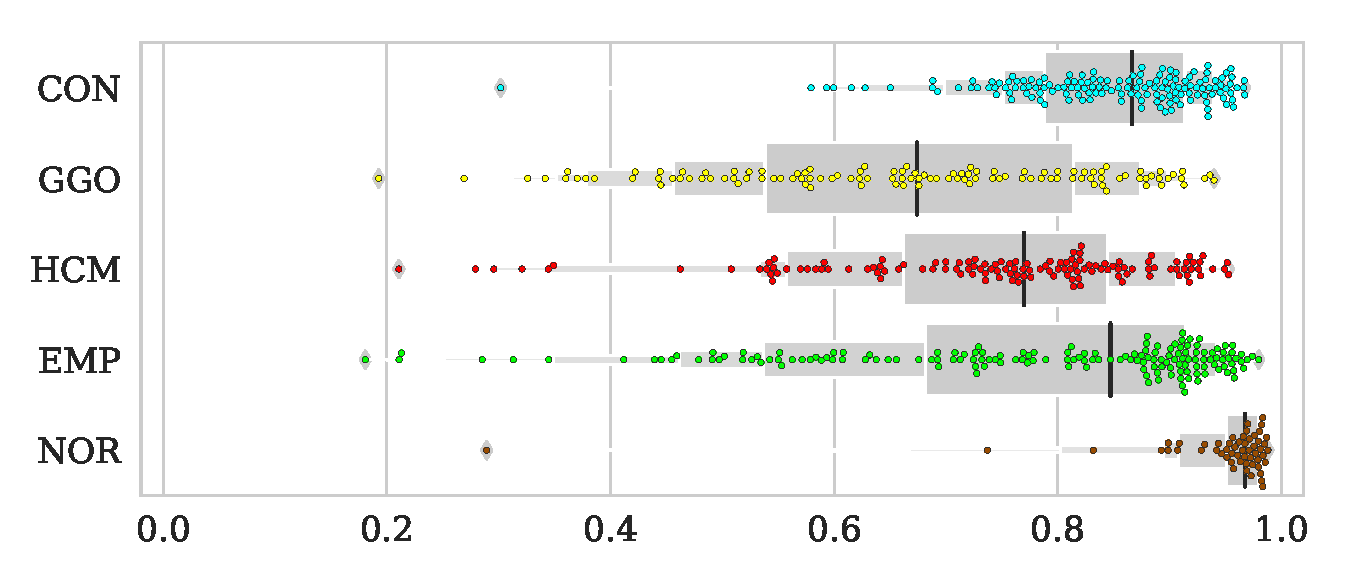
\includegraphics[width=\linewidth]{swarm_plot/plot.eps}
      \captionof{figure}{Swarm plot on top of a letter value plot of the dice coefficient for the proposed method ($\lambda=0.1$).}
      \label{dice_swarm}
    \end{minipage}
    \hfill
    \begin{minipage}[c]{.4\textwidth}
      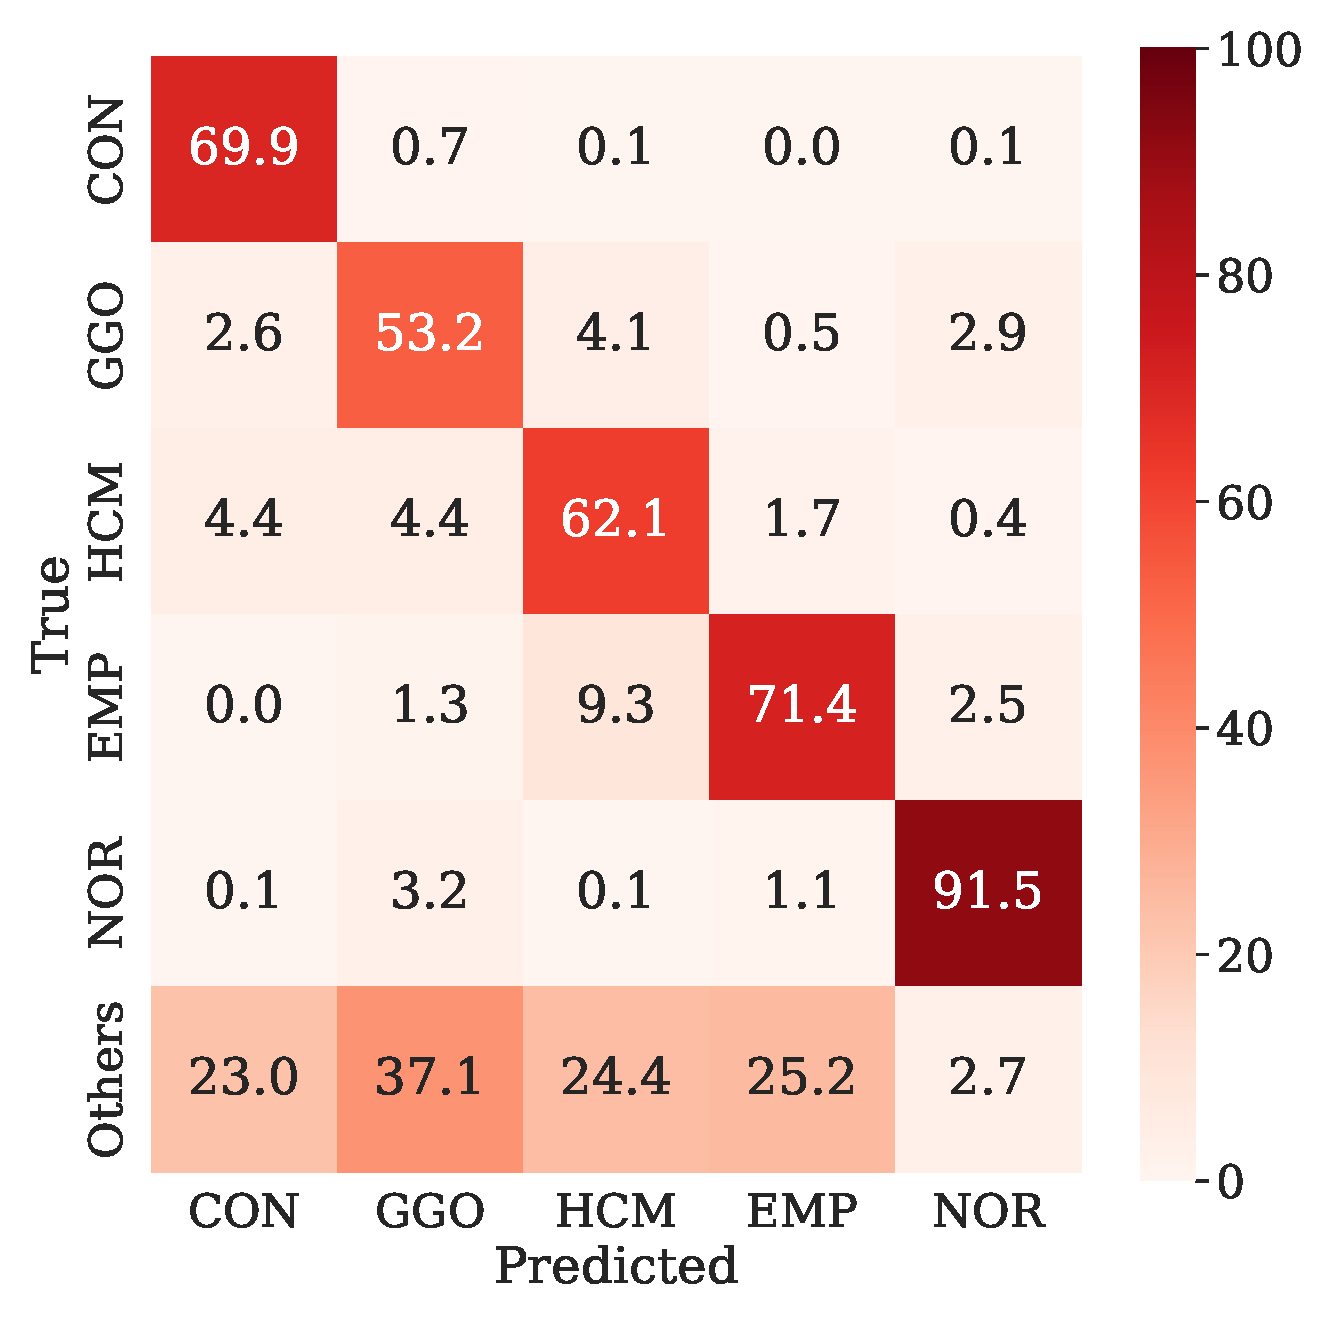
\includegraphics[width=\linewidth]{confusion_matrix/cm.eps}
      \caption{Confusion matrix for the proposed method ($\lambda=0.1$). Values are normalized along Y axis thus diagonal elements indicate the precisions.}
      \label{confusion_matrix}
    \end{minipage}
    \hfill
    \mbox{}
  \end{center}
\end{figure}

\newcommand{\vertical}[1]{\rotatebox[origin=c]{90}{#1}}
\begin{figure}[htbp]
  \begin{tabular}{ccccc}
    & Ground truth & Supervised only &  Proposed ($\lambda=0.1$) & Proposed ($\lambda=1$) \\

    \vertical{CON \textcolor{cyan}{$\blacksquare$}} &
    \begin{minipage}[c]{.21\textwidth}
      \centering
      \includegraphics[width=1\textwidth]{images/median/truth/1_0764_20080619_2_495.png}
    \end{minipage} &
    \begin{minipage}[c]{.21\textwidth}
      \centering
      \includegraphics[width=1\textwidth]{images/median/alpha0/1_0764_20080619_2_495.png}
    \end{minipage} &
    \begin{minipage}[c]{.21\textwidth}
      \centering
      \includegraphics[width=1\textwidth]{images/median/alpha0.1/1_0764_20080619_2_495.png}
    \end{minipage} &
    \begin{minipage}[c]{.21\textwidth}
      \centering
      \includegraphics[width=1\textwidth]{images/median/alpha1/1_0764_20080619_2_495.png}
    \end{minipage}
    \\
    & & 0.839 & 0.868 & 0.824
    \\
    \vertical{GGO \textcolor{yellow}{$\blacksquare$}} &
    \begin{minipage}[c]{.21\textwidth}
      \centering
      \includegraphics[width=1\textwidth]{images/median/truth/2_1134_20090216_3_145.png}
    \end{minipage} &
    \begin{minipage}[c]{.21\textwidth}
      \centering
      \includegraphics[width=1\textwidth]{images/median/alpha0/2_1134_20090216_3_145.png}
    \end{minipage} &
    \begin{minipage}[c]{.21\textwidth}
      \centering
      \includegraphics[width=1\textwidth]{images/median/alpha0.1/2_1134_20090216_3_145.png}
    \end{minipage} &
    \begin{minipage}[c]{.21\textwidth}
      \centering
      \includegraphics[width=1\textwidth]{images/median/alpha1/2_1134_20090216_3_145.png}
    \end{minipage}
    \\
    & & 0.693 & 0.676 & 0.876
    \\
    \vertical{HCM \textcolor{red}{$\blacksquare$}} &
    \begin{minipage}[c]{.21\textwidth}
      \centering
      \includegraphics[width=1\textwidth]{images/median/truth/3_0835_20080825_3_95.png}
    \end{minipage} &
    \begin{minipage}[c]{.21\textwidth}
      \centering
      \includegraphics[width=1\textwidth]{images/median/alpha0/3_0835_20080825_3_95.png}
    \end{minipage} &
    \begin{minipage}[c]{.21\textwidth}
      \centering
      \includegraphics[width=1\textwidth]{images/median/alpha0.1/3_0835_20080825_3_95.png}
    \end{minipage} &
    \begin{minipage}[c]{.21\textwidth}
      \centering
      \includegraphics[width=1\textwidth]{images/median/alpha1/3_0835_20080825_3_95.png}
    \end{minipage}
    \\
    & & 0.581 & 0.770 & 0.435
    \\
    \vertical{EMP \textcolor{green}{$\blacksquare$}} &
    \begin{minipage}[c]{.21\textwidth}
      \centering
      \includegraphics[width=1\textwidth]{images/median/truth/4_0222_20070621_3_180.png}
    \end{minipage} &
    \begin{minipage}[c]{.21\textwidth}
      \centering
      \includegraphics[width=1\textwidth]{images/median/alpha0/4_0222_20070621_3_180.png}
    \end{minipage} &
    \begin{minipage}[c]{.21\textwidth}
      \centering
      \includegraphics[width=1\textwidth]{images/median/alpha0.1/4_0222_20070621_3_180.png}
    \end{minipage} &
    \begin{minipage}[c]{.21\textwidth}
      \centering
      \includegraphics[width=1\textwidth]{images/median/alpha1/4_0222_20070621_3_180.png}
    \end{minipage}
    \\ & & 0.793 & 0.847 & 0.815
    \\
    \vertical{NOR \textcolor{brown}{$\blacksquare$}} &
    \begin{minipage}[c]{.21\textwidth}
      \centering
      \includegraphics[width=1\textwidth]{images/median/truth/5_0440_20070830_2_407.png}
    \end{minipage} &
    \begin{minipage}[c]{.21\textwidth}
      \centering
      \includegraphics[width=1\textwidth]{images/median/alpha0/5_0440_20070830_2_407.png}
    \end{minipage} &
    \begin{minipage}[c]{.21\textwidth}
      \centering
      \includegraphics[width=1\textwidth]{images/median/alpha0.1/5_0440_20070830_2_407.png}
    \end{minipage} &
    \begin{minipage}[c]{.21\textwidth}
      \centering
      \includegraphics[width=1\textwidth]{images/median/alpha1/5_0440_20070830_2_407.png}
    \end{minipage}
    \\
    & & 0.978 & 0.968 & 0.974
    \\

  \end{tabular}
  \caption{Average results and dice coefficients for each DLD pattern.
    Automated segmentation results are superimposed with colors.
    For each DLD pattern, the slice that gave the median dice coefficient for the proposed method with $\lambda=0.1$ was chosen to represent the average result.
    Note that although CNN performed multi-class segmentation, only one DLD pattern per slice was taken into account for the evaluation.}
  \label{average_results}
\end{figure}
